\documentclass[tikz,border=10pt]{standalone}
\usepackage{amsmath}
\usetikzlibrary{angles}

\begin{document}

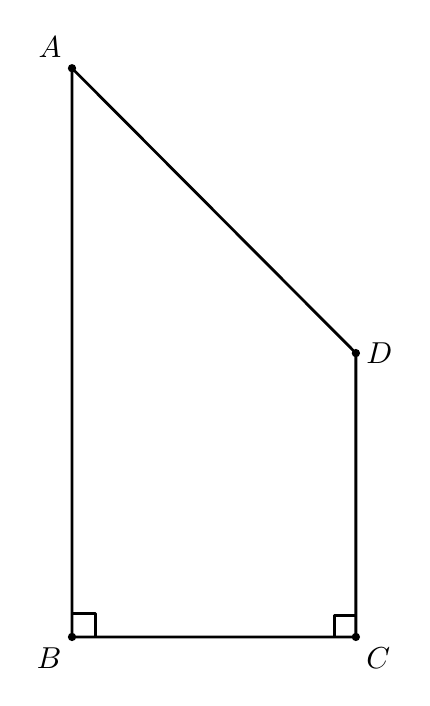
\begin{tikzpicture}[line width=1.0pt, line join=round]
\coordinate (A) at (-1.822,3.624);
\coordinate (B) at (-1.822,-3.599);
\coordinate (C) at (1.783,-3.599);
\coordinate (D) at (1.783,0.006);

  
  \draw (A) -- (B) -- (C) -- (D) -- (A);

  
  \draw pic[draw, angle radius=0.297cm] {right angle=A--B--C};
  \draw pic[draw, angle radius=0.271cm] {right angle=B--C--D};

  
  \fill (A) circle (1.500pt);
  \fill (B) circle (1.500pt);
  \fill (C) circle (1.500pt);
  \fill (D) circle (1.500pt);

  
  \node[above left] at (A) {\fontsize{10.5}{12.6}\selectfont $A$};
  \node[below left] at (B) {\fontsize{10.5}{12.6}\selectfont $B$};
  \node[below right] at (C) {\fontsize{10.5}{12.6}\selectfont $C$};
  \node[right] at (D) {\fontsize{10.5}{12.6}\selectfont $D$};
\end{tikzpicture}
\end{document}